\section{Temporal Action Proposals}
\par The task of Temporal Action Proposals involves generating temporal segments in long untrimmed video. Given a video, the model should be able to output temporal intervals (timestamps) that have a possibility of containing an action. Buch \textit{et al} \cite{buch2017sst} used Single-Stream Temporal Action Proposal (SST) that does not require division of input video into a number of short clips or use of overlapping sliding windows. The method uses a GRU-based sequence encoder which processes the video in a single pass and at each time step outputs proposals and their confidences by utilizing the C3D encoded features of the video frames. The model however had an issue of predicting an output segment which contains several ground-truth segments. Lin \textit{et al} \cite{lin2019bmn} develop a Boundary-Matching Mechanism for efficiently evaluating the proposals from a bottom-up generators and give reliable confidence scores.

\section{Transformers in Computer Vision}
\par Transformers \cite{tfm} have been widely used in applications requiring processing of sequential data like language or speech. Various solutions have been coming forward to utilize this generalized architectures in the domain of computer vision. Dosovitskiy \textit{et al} \cite{dosovitskiy2020vit} used only transformers (called Vision Transformers or ViT), without any CNN backbone for the task of image classification. The model divided an image into fixed-size patches and pass them along with an extra learnable class embedding token as input to a tranformer encoder. The output of the class embedding token is then feed to a MLP head to get the output object class. The approach suffers from the issues of less scalability and larger running time, since the number of tokens is highly dependent on the input resolution of the image. Liu \textit{et al} \cite{liu2021swin} tackles these issues by intoducing a hierarchical transformer called Swin-Transformer. The method uses shifted windows to limit the attention computation to non-overlapping local windows. It decreases the quadratic complexity of ViT to linear comutational complexity with respect to the input image size. Fayyaz \textit{et al} \cite{fayyaz2021ats} introduces a parameter free Adaptive Token Sampling (ATS) module which can be plugged into any ViT models and reduce the GFLOPs without any additional training. The proposed method decides and selects the right amount of tokens to attend to. 
\par Carion \textit{et al} \cite{carion2020detr} develop DEtection TRansformer (DETR) for the task of object detection or panoptic segmentation in images. The method completely eradicates the need of developing various hand-designed features like anchors, non-max supression thresholds, etc. It is an end-to-end architecture viewing object detection task as set prediction task. The model tokenizes the input image using a CNN backbone (ResNet-50) and passes it to the transformer encoder along with positional embeddings. The output of encoder is given to the decoder along with learnable positional embeddings refered to as object queries. The decoder outputs the query features which are passed to a shared Feed Forward Network (FFN) that predicts the object bounding box and class. They use Hungarian Bipartite Matcher to compute the loss between ground truth and prediction. DETR inspite of comparable performance with other SOTA CNN architectures, faced issues of slower convergence because of global attention in encoder and inaccuracy in detection of smaller objects. A number of approaches were introduced for handling this issue. Zhu \textit{et al} \cite{zhu2020deformable} proposed Deformable DETR which answers both the issues by using Multi-scale Feature Maps of the input image and attending to limited number of tokens in encoder. The method also introduced variations for better accuracy, namely iterative bounding box refinement and two-stage Deformable DETR. The model required 10x faster convergence and is 1.6x faster than the original DETR. This however does increase the input tokens by 20x because of multi-scale features. Roh \textit{et al} \cite{roh2021sparse} make Deformable DETR further efficient by selectively updating only the tokens that are expected to be referenced by the DETR decoder. This is done by learning a scoring network for predicting binarized Decoder cross-Attention Map (DAM). The model also improves the gradient flow throughout the transformer by introducing encoder-auxiliary loss. Sparse-DETR along with Swin Transformer Backbone increases the FPS by 38\% as compared to Deformable DETR.


\section{Dense Video Captioning}
\par The problem of dense video captioning was introduced by Krishna \textit{et al} in \cite{krishna2017densecaptioning} by proposing ActivityNet Captions dataset. Their architecture involved a proposal module and captioning module. The proposal module was inspired from DAPs \cite{Escorcia2016DAPsDA}, while the captioning module incorporated LSTM with contextual features along with event feature as inputs. The architecture was able to detect events and generate captions of the video in a single pass without the need of a time consuming sliding window approach.  However, since the features were dependent on the end location of the event, the model generated same captions for events ending at same timestamp.

\begin{figure}[h]
	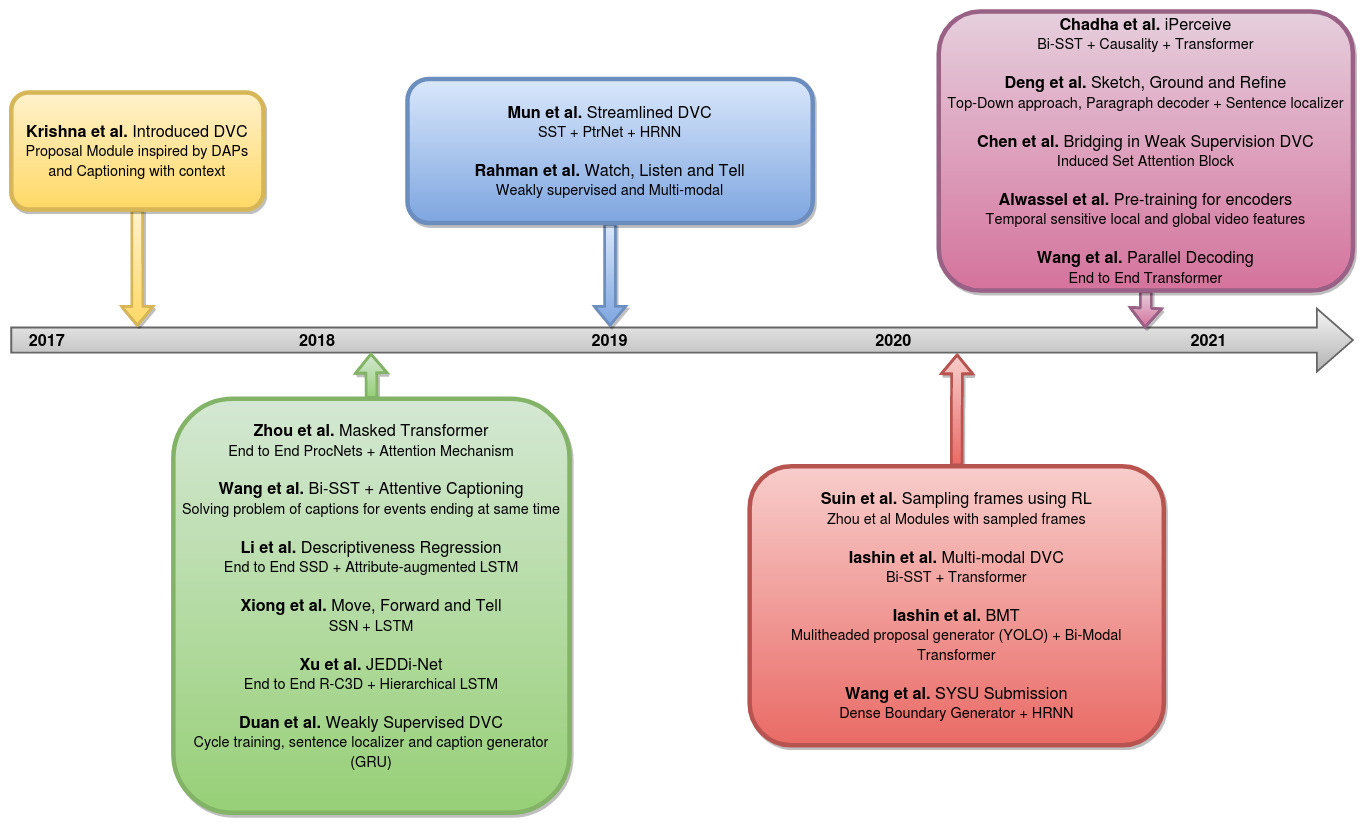
\includegraphics[width=\linewidth]{assets/img/timeline.jpg}
	\caption{Evolution of dense video captioning methods over time.}
\end{figure}

\par Following the release of ActivityNet Captions dataset in 2017, many researchers were able to surpass the results of baseline model and achieve state-of-the-art. Zhou \textit{et al} \cite{zhou2018end} addressed the problem of little influence of language desciptions on event proposals if the two modules are trained separately. They introduced an end-to-end masked transformer for propogating captioning error to proposal module for better performance. Furthermore, they proposed a self-attention mechanism for learning long-range dependencies in video. The proposal module was based on ProcNets \cite{zhou2017automatic}. The caption decoder employed a differentiable proposal mask to account for features in the respective event. Wang \textit{et al} \cite{wang2018bidirectional} employed Bi-SST as their proposal generator to account for past and future context information. The captioning module consisted of attentive fusion of context features, the weights of which were decided by a context gating mechanism. The architecture selected final captions based on joint ranking method which accounted for both proposal and caption confidence. Li \textit{et al} \cite{li2018jointly}, inspired by object localization networks like \cite{ren2016faster, liu2016ssd}, presented an end-to-end model with descriptiveness regression. An attribute-augmented LSTM network optimized using reinforcement learning was used for captioning module. Xiong \textit{et al} \cite{xiong2018forward} strived to generate relevant, coherent and concise descriptions using SSN \cite{zhao2017temporal} for event localization and LSTM for event selection and caption generation. Reinforcement learning with sentence-level reward is used to train the captioning network. Xu \textit{et al} \cite{xu2018joint} proposed JEDDi-Net, an end-to-end architecture incorporating visual and language contexts. Segment Proposal Network inspired from R-C3D \cite{xu2017rc3d} is used for proposal generation. Hierarchical LSTM with caption-level controller network and word-level sentence decoder is used for caption generation. The proposal features are represented using 3D Segment-of-Interest Pooling. Duan \textit{et al} \cite{duan2018weakly} introduced weak supervision training with no need of temporal annotations of events. They trained sentence localizer and caption generator in cyclic manner minimizing the reconstruction loss. However, the method struggles to detect beginning of events properly.

\par Mun \textit{et al} \cite{mun2019streamlined} tackles the challenge of coherent captioning by considering temporal dependency between events. They used SST for event proposals, PtrNet for event sequence generation and HRNN for captioning. Rahman \textit{et al} \cite{rahman2019watch} utilized weak supervision method from \cite{duan2018weakly} and were the first to try multi-modal approach for dense video captioning. They show how audio alone can be competitive to the previous visual based results. The paper also discusses various methods to encode audio (MFCC, CQT, SoundNet) and context fusion techniques for multiple modalities (Multiplicative Mixture, Multi-modal context fusion, MUTAN). The architecture suffered from proposal localization accuracy due to weak supervision. Furthermore, the results are also affected due to unavailability of part of the dataset as some videos are not available on their respective urls.

\par \sloppy Suin \textit{et al} \cite{suin2020efficient} aimed to reduce computational cost by processing fewer frames. They used deep reinforcement-based approach to describe multiple events in a video by watching a portion of the frames. The event proposal and captioning modules were inspired from \cite{zhou2018end}. Iashin \textit{et al} \cite{iashin2020multimodal} shows the importance of audio and speech modalities alongside visual features for dense video captioning task. They employ a Bi-SST for proposal and the captioning module consists of a Transformer architecture with three blocks: an encoder, decoder and generator. The model was able to achieve better performance than the then existing methods despite of unavailability of full dataset for multiple modalities. Iashin \textit{et al} \cite{iashin2020better} utilized audio and video with Bi-modal Transformer for captioning. The proposal generator consisted of multiheaded method, inspired from YOLO object detector \cite{yolo}. Their ablation analysis depicted stronger contribution of visual cues alone than audio cues alone. However, both modalities combined gave better results. Wang \textit{et al} \cite{wang2020densecaptioning} adapt DBG \cite{lin2019fast} for temporal event proposals alongwith ESGN \cite{mun2019streamlined} for candidate subset selection. The captioning module consists of an encoder-decoder architecture with CMG (cross-modal gating) block to adaptively balance the visual and linguistic information.

\par Chadha \textit{et al} \cite{chadha2020iperceive} proposed to handle cognitive error (causality between events) and incorrect attention (attending to objects in the frame). Their end-to-end model consisted of Bi-SST for proposals, Common-Sense Reasoning for causality learning and Transformer based architecture \cite{iashin2020multimodal} for captioning. The common-sense reasonining module employed a borrow-put experiment for determining dependency between events and generate context-aware features. Deng \textit{et al} \cite{deng2021sketch} introduced a top-down approach, reversing the usual detect-then-describe method. The architecture first generates a multi-sentence paragraph to describe the whole video and then localize each sentence for events. The captions are then refined using dual-path cross attention module. The top-down approach increased coherency in captions. Chen \textit{et al} \cite{chen2021towards} worked on closely bridging event localization and captioning modules for weakly supervised learning. The Induced Set Attention Block helps the captioner to learn highly abstracted global structure of the video. The method suffers from detecting visually small concepts/objects. Alwassel \textit{et al} \cite{alwassel2021tsp} introduce a supervised pre-training  paradigm for temporal action localization. The paradigm also considers background clips and global video information, to improve temporal sensitivity. Wang \textit{et al} \cite{wang2021endtoend} formulated dense video captioning as a set prediction task and introduced an end-to-end dense video captioning framework with parallel decoding (PDVC). PDVC adopts the vision transformer to learn attentive interaction of different frames. Two prediction heads run in parallel over query features, leveraging the mutual benefits between two tasks of localization and captioning.

% Please add the following required packages to your document preamble:
% \usepackage{multirow}
\begin{table}[]
	\begin{tabular}{|c|c|cccc|cccc|}
		\hline
		\multirow{2}{*}{\textbf{Paper}}          & \multirow{2}{*}{\textbf{Set}} & \multicolumn{4}{c|}{\textbf{Ground Truth Proposals}}                                                                          & \multicolumn{4}{c|}{\textbf{Learnt Proposals}}                                                                       \\ \cline{3-10} 
		&                               & \multicolumn{1}{c|}{\textbf{M}} & \multicolumn{1}{c|}{\textbf{C}} & \multicolumn{1}{c|}{\textbf{B@3}} & \textbf{B@4}          & \multicolumn{1}{c|}{\textbf{M}} & \multicolumn{1}{c|}{\textbf{C}} & \multicolumn{1}{c|}{\textbf{B@3}} & \textbf{B@4} \\ \hline
		\multirow{2}{*}{Krishna \textit{et al} \cite{krishna2017densecaptioning} DCE}             & Validation                    & \multicolumn{1}{c|}{8.88}       & \multicolumn{1}{c|}{25.12}      & \multicolumn{1}{c|}{4.09}         & 1.60                  & \multicolumn{1}{c|}{5.69}       & \multicolumn{1}{c|}{12.43}      & \multicolumn{1}{c|}{1.90}         & 0.71         \\ \cline{2-10} 
		& Test                          & \multicolumn{1}{c|}{9.46}       & \multicolumn{1}{c|}{24.56}      & \multicolumn{1}{c|}{7.12}         & 3.98                  & \multicolumn{1}{c|}{4.82}       & \multicolumn{1}{c|}{17.29}      & \multicolumn{1}{c|}{3.86}         & 2.20         \\ \hline
		\multirow{2}{*}{Zhou \textit{et al} \cite{zhou2018end} Masked Transformer} & Validation                    & \multicolumn{1}{c|}{11.16}      & \multicolumn{1}{c|}{47.71}      & \multicolumn{1}{c|}{5.76}         & 2.71                  & \multicolumn{1}{c|}{4.98}       & \multicolumn{1}{c|}{9.25}       & \multicolumn{1}{c|}{2.42}         & 1.15         \\ \cline{2-10} 
		& Test                          & \multicolumn{1}{c|}{10.12}      & \multicolumn{1}{c|}{}           & \multicolumn{1}{l|}{}             & \multicolumn{1}{l|}{} & \multicolumn{1}{c|}{10.12}      & \multicolumn{1}{l|}{}           & \multicolumn{1}{c|}{}             &              \\ \hline
		\multirow{2}{*}{Wang \textit{et al} \cite{wang2018bidirectional} Bi-SST}             & Validation                    & \multicolumn{1}{c|}{10.89}      & \multicolumn{1}{c|}{}           & \multicolumn{1}{c|}{}             &                       & \multicolumn{1}{c|}{5.86}       & \multicolumn{1}{c|}{7.99}       & \multicolumn{1}{c|}{2.55}         & 1.31         \\ \cline{2-10} 
		& Test                          & \multicolumn{1}{c|}{}           & \multicolumn{1}{c|}{}           & \multicolumn{1}{l|}{}             & \multicolumn{1}{l|}{} & \multicolumn{1}{c|}{9.65}       & \multicolumn{1}{l|}{}           & \multicolumn{1}{c|}{}             &              \\ \hline
		\multirow{2}{*}{Li \textit{et al} \cite{li2018jointly} Descriptivness Regr.} & Validation                    & \multicolumn{1}{c|}{10.33}      & \multicolumn{1}{c|}{26.26}      & \multicolumn{1}{c|}{4.55}         & 1.71                  & \multicolumn{1}{c|}{6.93}       & \multicolumn{1}{c|}{13.21}      & \multicolumn{1}{c|}{2.27}         & 0.74         \\ \cline{2-10} 
		& Test                          & \multicolumn{1}{c|}{}           & \multicolumn{1}{c|}{}           & \multicolumn{1}{l|}{}             & \multicolumn{1}{l|}{} & \multicolumn{1}{c|}{12.96}      & \multicolumn{1}{l|}{}           & \multicolumn{1}{c|}{}             &              \\ \hline
		Xu \textit{et al} \cite{xu2018joint} JEDDi-Net                             & Test                          & \multicolumn{1}{c|}{}           & \multicolumn{1}{c|}{}           & \multicolumn{1}{c|}{4.06}         & 1.63                  & \multicolumn{1}{c|}{8.58}       & \multicolumn{1}{c|}{19.88}      & \multicolumn{1}{c|}{4.06}         & 1.63         \\ \hline
		\multirow{2}{*}{Mun \textit{et al} \cite{mun2019streamlined} Streamlined DVC}     & Validation                    & \multicolumn{1}{c|}{13.07}      & \multicolumn{1}{c|}{43.48}      & \multicolumn{1}{c|}{4.41}         & 1.28                  & \multicolumn{1}{c|}{8.82}       & \multicolumn{1}{c|}{30.68}      & \multicolumn{1}{c|}{2.94}         & 0.93         \\ \cline{2-10} 
		& Test                          & \multicolumn{1}{c|}{}           & \multicolumn{1}{c|}{}           & \multicolumn{1}{l|}{}             & \multicolumn{1}{l|}{} & \multicolumn{1}{c|}{8.19}       & \multicolumn{1}{l|}{}           & \multicolumn{1}{c|}{}             &              \\ \hline
		Duan \textit{et al} \cite{duan2018weakly} Weakly Supervised DCE               & Test                          & \multicolumn{1}{c|}{}           & \multicolumn{1}{c|}{}           & \multicolumn{1}{c|}{2.62}         & 1.27                  & \multicolumn{1}{c|}{6.3}        & \multicolumn{1}{c|}{18.77}      & \multicolumn{1}{c|}{2.62}         & 1.27         \\ \hline
		Rahman \textit{et al} \cite{rahman2019watch} Watch, Listen, Tell               & Validation *                  & \multicolumn{1}{c|}{7.23}       & \multicolumn{1}{c|}{25.36}      & \multicolumn{1}{c|}{3.04}         & 1.46                  & \multicolumn{1}{c|}{4.93}       & \multicolumn{1}{c|}{13.79}      & \multicolumn{1}{c|}{1.85}         & 0.9          \\ \hline
		Suin \textit{et al} \cite{suin2020efficient} Efficient framework for DVC         & Validation                    & \multicolumn{1}{c|}{}           & \multicolumn{1}{c|}{}           & \multicolumn{1}{c|}{2.87}         & 1.35                  & \multicolumn{1}{c|}{6.21}       & \multicolumn{1}{c|}{13.82}      & \multicolumn{1}{c|}{2.87}         & 1.35         \\ \hline
		Iashin \textit{et al} \cite{iashin2020multimodal} Multi-modal DVC                   & Validation *                  & \multicolumn{1}{c|}{11.72}      & \multicolumn{1}{c|}{}           & \multicolumn{1}{c|}{5.83}         & 2.86                  & \multicolumn{1}{c|}{7.31}       & \multicolumn{1}{l|}{}           & \multicolumn{1}{c|}{2.6}          & 1.07         \\ \hline
		Iashin \textit{et al} \cite{iashin2020better} BMT                               & Validation *                  & \multicolumn{1}{c|}{10.90}      & \multicolumn{1}{c|}{}           & \multicolumn{1}{c|}{4.63}         & 1.99                  & \multicolumn{1}{c|}{8.44}       & \multicolumn{1}{l|}{}           & \multicolumn{1}{c|}{3.84}         & 1.88         \\ \hline
		Xiong \textit{et al} \cite{xiong2018forward} Move Forward and Tell              & Validation                    & \multicolumn{1}{c|}{}           & \multicolumn{1}{c|}{}           & \multicolumn{1}{c|}{2.84}         & 1.24                  & \multicolumn{1}{c|}{7.08}       & \multicolumn{1}{l|}{}           & \multicolumn{1}{c|}{2.84}         & 1.24         \\ \hline
		\multirow{2}{*}{Wang \textit{et al} \cite{wang2020densecaptioning} SYSU}               & Validation                    & \multicolumn{1}{c|}{14.85}      & \multicolumn{1}{c|}{}           & \multicolumn{1}{l|}{}             & \multicolumn{1}{l|}{} & \multicolumn{1}{c|}{10.31}      & \multicolumn{1}{l|}{}           & \multicolumn{1}{c|}{}             &              \\ \cline{2-10} 
		& Test                          & \multicolumn{1}{c|}{}           & \multicolumn{1}{c|}{}           & \multicolumn{1}{l|}{}             & \multicolumn{1}{l|}{} & \multicolumn{1}{c|}{9.28}       & \multicolumn{1}{l|}{}           & \multicolumn{1}{c|}{}             &              \\ \hline
		Chadha \textit{et al} \cite{chadha2020iperceive} iPerceive                         & Validation *                  & \multicolumn{1}{c|}{12.27}      & \multicolumn{1}{c|}{}           & \multicolumn{1}{c|}{6.13}         & 2.98                  & \multicolumn{1}{c|}{7.87}       & \multicolumn{1}{l|}{}           & \multicolumn{1}{c|}{2.93}         & 1.29         \\ \hline
		Deng \textit{et al} \cite{deng2021sketch} Sketch, Ground and Refine           & Validation                    & \multicolumn{1}{c|}{}           & \multicolumn{1}{c|}{}           & \multicolumn{1}{l|}{}             & 1.67                  & \multicolumn{1}{c|}{9.37}       & \multicolumn{1}{c|}{22.12}      & \multicolumn{1}{c|}{}             & 1.67         \\ \hline
		Chen \textit{et al} \cite{chen2021towards} Towards Bridging EC-SL              & Validation                    & \multicolumn{1}{c|}{}           & \multicolumn{1}{c|}{}           & \multicolumn{1}{c|}{2.78}         & 1.33                  & \multicolumn{1}{c|}{7.49}       & \multicolumn{1}{c|}{21.21}      & \multicolumn{1}{c|}{2.78}         & 1.33         \\ \hline
		\textbf{Alwassel \textit{et al} \cite{alwassel2021tsp} TSP with BMT}           & Validation                    & \multicolumn{1}{c|}{}           & \multicolumn{1}{c|}{}           & \multicolumn{1}{c|}{4.16}         & 2.02                  & \multicolumn{1}{c|}{8.75}       & \multicolumn{1}{l|}{}           & \multicolumn{1}{c|}{4.16}         & 2.02         \\ \hline
		Wang \textit{et al} \cite{wang2021endtoend} Parallel decoding                   & Validation *                  & \multicolumn{1}{c|}{11.26}      & \multicolumn{1}{c|}{53.65}      & \multicolumn{1}{l|}{}             & 3.12                  & \multicolumn{1}{c|}{8.08}       & \multicolumn{1}{c|}{28.59}      & \multicolumn{1}{c|}{}             & 1.96         \\ \hline
	\end{tabular}

\centering
\caption{Performance comparison of previous methods on the ActivityNet Captions dataset (* some videos unavailable)}  \label{tab: performance-comparison}

\end{table}

\section{Identified Themes}
\par Dense video captioning can be decomposed into two parts: event localization and event description. Existing research methodologies can be grouped into different categories based on training methods, modalities used and ordering of tasks.

\subsection{Based on Training schemes}
\begin{enumerate}
	\item \textbf{Independent training}: Training the proposal and captioning module independently, with no loss propogation or interaction between the two.
	\item \textbf{Alternate training}: alternate between i) training the proposal module only and ii) training the captioning module on the positive event proposals while fine-tuning the proposal module.
	\item \textbf{End-to-End}: Training the proposal and captioning module together, with caption information being able to affect and improve localization capability in the video.
	\item \textbf{Weakly Supervised}: Training the model without ground-truth annotations of temporal events. This method assumes one-to-one correspondence between i.e. each caption describes one temporal event, and each temporal event has one caption.
\end{enumerate}

\subsection{Based on Modalities}
\begin{enumerate}
	\item \textbf{Uni-modal}: Utilizes only one type of input feature. For example, only visual features.
	\item \textbf{Multi-modal}: Utilizes more than one type of input features. For example, combinations of visual, audio and speech features.
\end{enumerate}

\subsection{Based on Task ordering}
\begin{enumerate}
	\item \textbf{Top-Down}: \textit{localize-then-describe}. Predicts the temporal intervals and then caption them. May include optional postprocessing such as ranking proposals, extracting top-k proposals based on confidence scores, etc.
	\item \textbf{Bottom-Up}: \textit{describe-localize-refine}. Describes the entire video into a paragraph using Video Paragraph Generation models. Then localize each sentence from the paragraph over the video. The localized boundaries are then used to re-caption the event.
\end{enumerate}

\section{Research Literature Gaps}
\subsection{Less Explored}
\par The research on dense video captioning task is still on its early stage of development. There has been extensive work done in the field of computer vision on tasks like image classification, object localization and detection, image captioning, action classification on short video clips spanning few tens of seconds, etc. The computation costs in processing and cost of annotating long untrimmed videos is a major reason of less development in the field. Though research has been done on tasks like video summarization with a paragraph in the field of NLP, the models only utilizes the language features and completely discards the visual modality which can be very helpful in describing meaningful captions which cannot be captured by sole speech. 

\subsection{Use of Transformers}
\par The existing research mostly utilizes CNN based models for feature extraction and proposal generation, given its performance legacy in image related tasks. The CNN based architectures require additional hand crafted components like anchor selection based on appearance and distribution of object to be predicted in the dataset, threshold for non-max supression to remove redundant predictions or multiple processing stages (eg. label generation) to detect arbitrarily shaped objects. Transformers on the other hand are more general architectures and have low inductive bias. Their structure has the capability to run on different modalities with very little modifications across modalitites. With large amount of image and video data available across internet, transformer have the potential to become the state-of-the-art methods in computer vision due to their better generalizability.

\subsection{Multimodal architecture}
\par The invention of Neural Networks is greatly inspired by the way human brain processes visual data and its ability to learn to recognize objects. Information in the real world usually comes as different modalities. Humans also utilize multiple modalities for processing and leanring things. Majority of research work in DVC utilizes single modality of either just video frames or just speech. Thus it is important to design models that are able to jointly respresent information from different modalities and make decision according to it.

\subsection{Efficient Attention mechanisms}
\par Although there are many benefits of utilizing transformers, there are few concerns too. Transformers takes longer execution times for training and inference as compared to their CNN counterparts. The attention in transformer has quadratic complexity with respect to the number of input tokens. And the tokens in computer vision tasks are much larger than that in case of language tasks. These requires many decisions like input resolution and sliding stride size along both spatial and temporal dimension for feature generation. This will in turn affect the size of predicted objects or events. Hence methods are needed to reduce the execution time by smart selection of tokens for attention.

\subsection{End-to-End training}
\par The video event segments and language are closely related and the caption information should be able to help localize temporal events in the video. Using independent or alternate training of modules disregards this relationship and predict inferior timestamps and captions. On the other hand, end-to-end training mechanisms allow proper gradient flow across modules and help in generating rich predictions.
